%-----------------------------
\section{Minimum Spanning Tree (MST)}

\subsection{Problem}


\begin{frame}
\frametitle{Minimum Spanning Tree (MST)}
\begin{block}{Problemstellung}
\begin{itemize}
\item „finde das billigste Netzwerk“
\item genau: \\
Gegeben sei ein zusammenhängender ungerichteter gewichteter Graph, gesucht ist ein Spannbaum mit geringstem Gesamtgewicht.
\end{itemize}
\end{block}

\end{frame}

\begin{frame}
\frametitle{Minimum Spanning Tree (MST)}
\begin{block}{Lösung}
\begin{itemize}
\item Ansatz: baue einen Baum mit greedy Algorithmus:
\begin{enumerate}
\item betrachte Kante mit niedrigstem Gewicht
\item untersuche: führt hinzufügen der Kante zu einem Zyklus?
\begin{itemize}
\item Ja: verwerfe Kante
\item Nein: füge Kante zum Baum hinzu
\end{itemize}
\item starte bei 1. mit restlichen Kanten bis alle abgearbeitet sind
\item $ \implies $ Baum ist ein MST
\end{enumerate}
\end{itemize}
\end{block}

\end{frame}

\begin{frame}
\frametitle{Lösung}
\begin{figure}
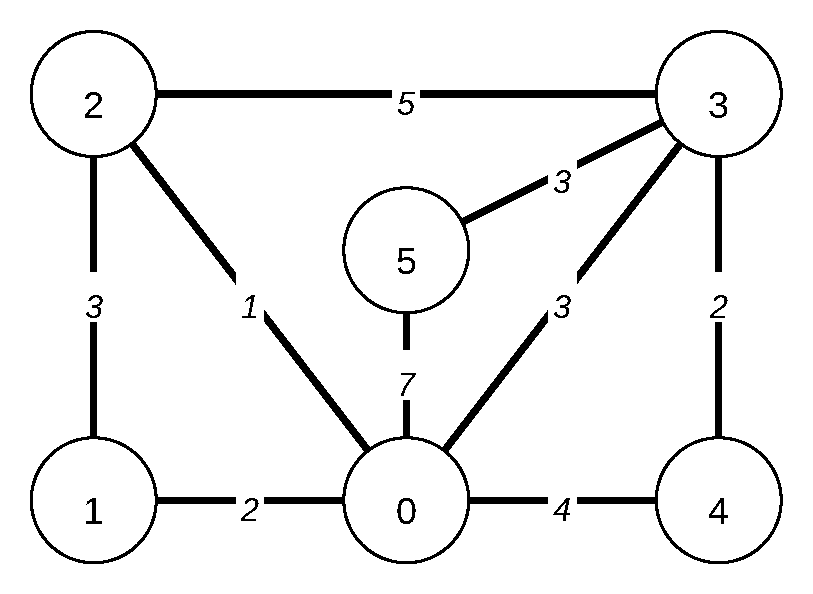
\includegraphics[width=0.75\linewidth, trim = 2mm 2mm 2mm 2mm, clip = true]{kruskal_graphs/graph1.pdf}
\end{figure}
\end{frame}

\begin{frame}
\frametitle{Lösung}
\begin{figure}
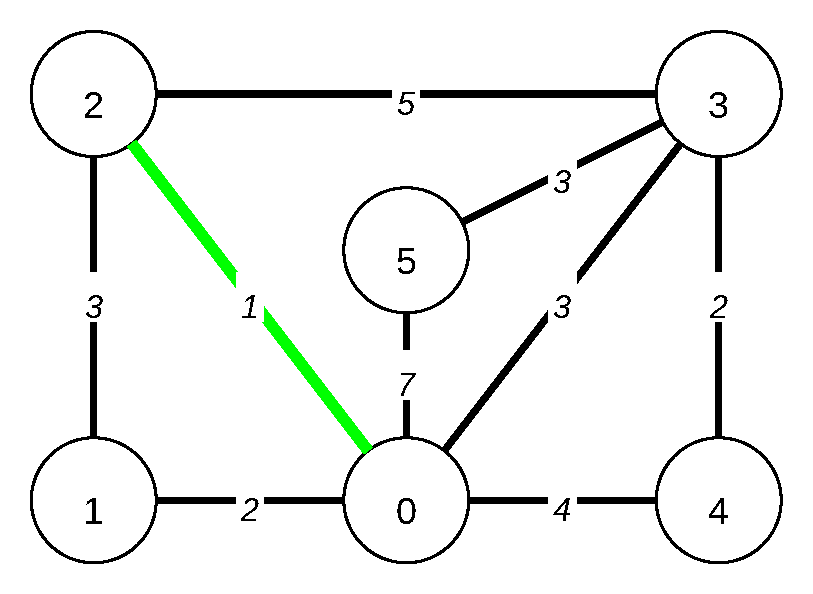
\includegraphics[width=0.75\linewidth, trim = 2mm 2mm 2mm 2mm, clip = true]{kruskal_graphs/graph2.pdf}
\end{figure}
\end{frame}

\begin{frame}
\frametitle{Lösung}
\begin{figure}
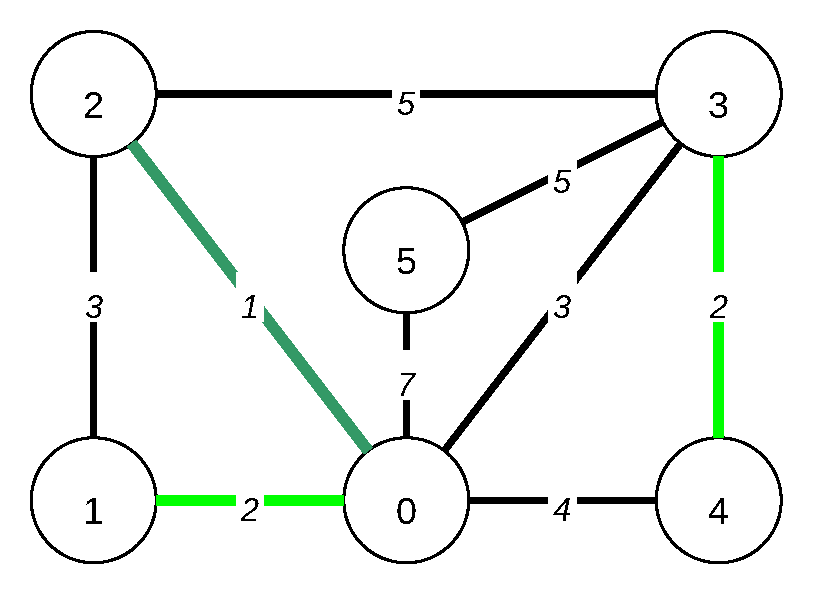
\includegraphics[width=0.75\linewidth, trim = 2mm 2mm 2mm 2mm, clip = true]{kruskal_graphs/graph3.pdf}
\end{figure}
\end{frame}

\begin{frame}
\frametitle{Lösung}
\begin{figure}
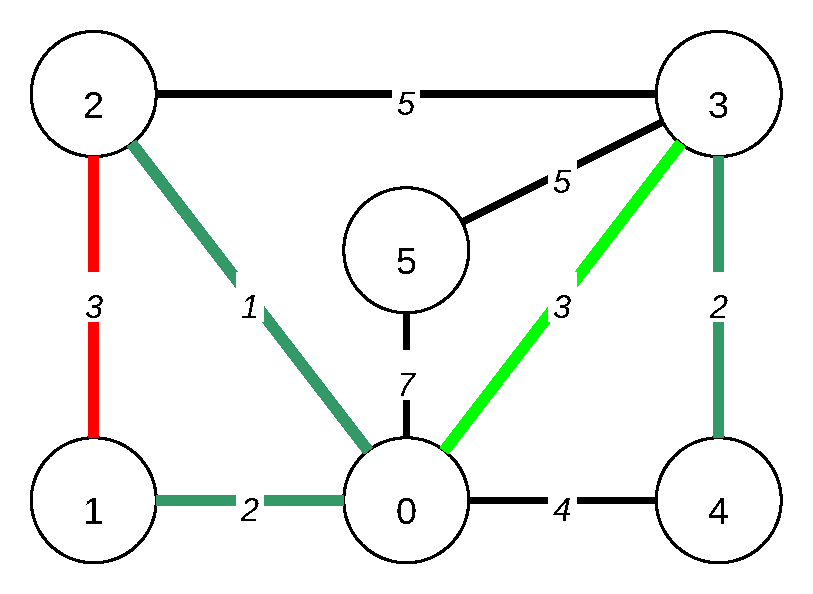
\includegraphics[width=0.75\linewidth, trim = 2mm 2mm 2mm 2mm, clip = true]{kruskal_graphs/graph4.pdf}
\end{figure}
\end{frame}

\begin{frame}
\frametitle{Lösung}
\begin{figure}
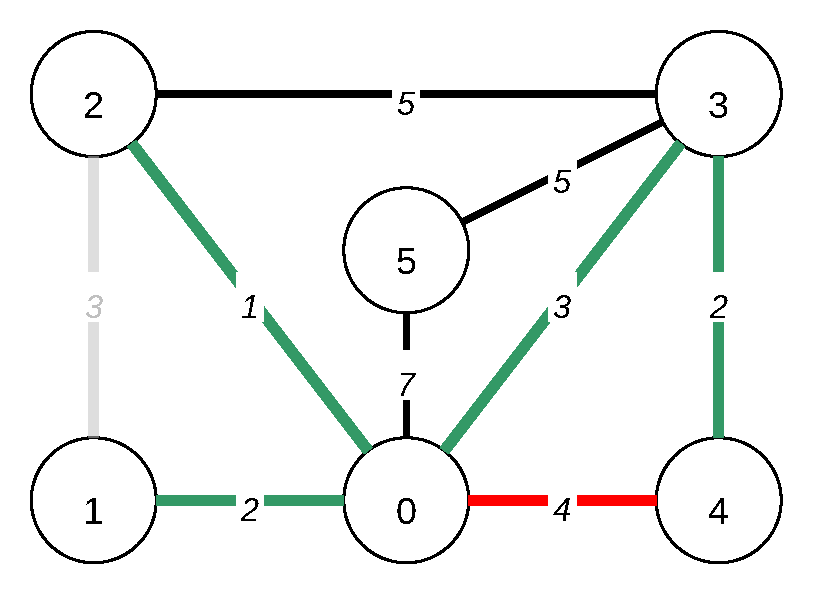
\includegraphics[width=0.75\linewidth, trim = 2mm 2mm 2mm 2mm, clip = true]{kruskal_graphs/graph5.pdf}
\end{figure}
\end{frame}

\begin{frame}
\frametitle{Lösung}
\begin{figure}
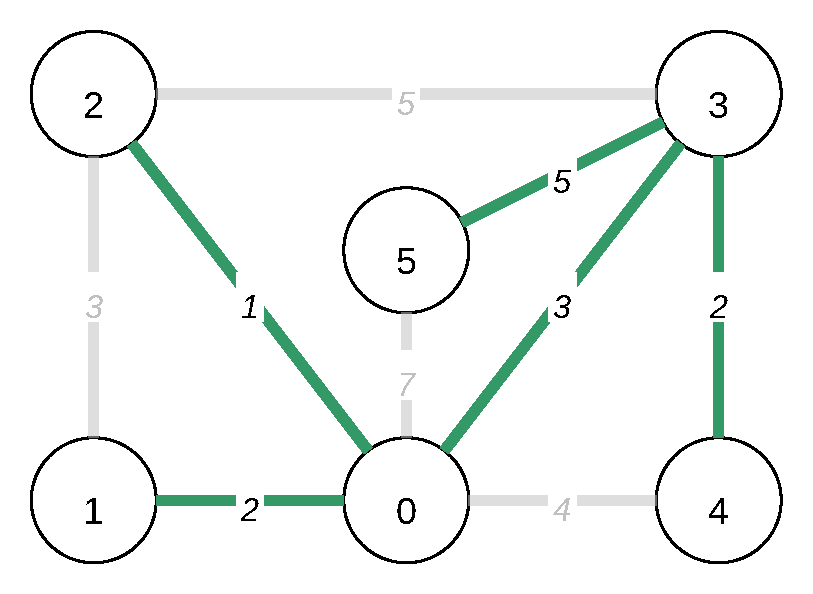
\includegraphics[width=0.75\linewidth, trim = 2mm 2mm 2mm 2mm, clip = true]{kruskal_graphs/graph6.pdf}
\end{figure}
\end{frame}

\subsection{Lösung: Kruskal}

\begin{frame}
\frametitle{Kruskal}
\begin{block}{Implementierung - Algorithmus von Kruskal}
\begin{itemize}
\item sortiere Kanten nach Gewicht
\item benutze Union-Find um Zyklen zu detektieren
\end{itemize}
\end{block}
\end{frame}


\begin{frame}[fragile]
\frametitle{Kruskal}
\begin{lstlisting}[basicstyle=\footnotesize]
int kruskal(std::vector<edge>& edges, int maxnode) {
    int fullweight = 0;
    UnionFind ufind(maxnode + 1);
    std::sort(edges.begin(), edges.end());
    for (const auto& e : edges) {
        if(!ufind.sameSet(e.from, e.to)) {
            ufind.unify(e.from, e.to);
            fullweight += e.weight;
        }
    }
    return fullweight;
}
\end{lstlisting}
\end{frame}

\begin{frame}
\frametitle{Kruskal}
Für Laufzeiten: $n:=|V|$, $m:=|E|$ \\~\\
\begin{block}{Laufzeit}
$\ O(m\log(m)+ m\cdot\alpha(n))=O(m\log(m))$\\$\ =O(m\log(n^2))=O(2m\log(n))=O(m\log(n))$

\end{block}
\end{frame}


\begin{frame}
\frametitle{Kruskal}
\begin{block}{Weitere lösbare Probleme}
\begin{itemize}
\item Maximum Spanning Tree
\item „MST" finden, wenn Kanten vorgegeben sind
\item Minimum Spanning Forest: mehrere getrennte Bäume
\item Minimax-Problem:
\begin{itemize}
\item Finden des Pfades zwischen zwei Knoten mit dem kleinsten Maximalgewicht einer Kante
\end{itemize}
\end{itemize}
\end{block}
\end{frame}
